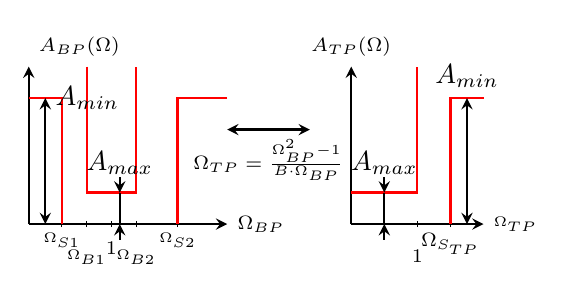
\begin{tikzpicture}[xscale=0.21, yscale=0.2]
% BP
\begin{scope}[local bounding box=BP]
	% Achsen zeichnen
	\draw[-{stealth},thick] (0,0) -- (12,0) node[right] {\scriptsize{$\Omega_{BP}$}};
	\draw[-{stealth},thick] (0,0) -- (0,10) node[above right] {\scriptsize{$A_{BP}(\Omega)$}};
	% Achsen beschriften
	\draw (2,-.2) -- (2,.2) node[below=1pt] {\tiny{$\Omega_{S1}$}};
	\draw (3.5,-.2) -- (3.5,.2) node[below=7pt] {\tiny{$\Omega_{B1}$}};
	\draw (5,-.2) -- (5,.2) node[below=4pt] {\scriptsize{$1$}};
	\draw (6.5,-.2) -- (6.5,.2) node[below=7pt] {\tiny{$\Omega_{B2}$}};
	\draw (9,-.2) -- (9,.2) node[below=1pt] {\tiny{$\Omega_{S2}$}};
	% BP-Teil zeichnen:
	\draw[color=red, thick] (2,0) -- (2,8) -- (0,8);
	\draw[color=red, thick] (3.5,10) -- (3.5,2) -- (6.5,2) -- (6.5,10);
	\draw[color=red, thick] (12,8) -- (9,8) -- (9,0); 
	\draw[{stealth}-{stealth}, thick] (1,0) -- (,8) node[right] {$A_{min}$};
	\draw[-{stealth}, thick] (5.5,-1) -- (5.5,0);
	\draw[{stealth}-, thick] (5.5,2) -- node[above] {$A_{max}$}(5.5,3);
	\draw[thick] (5.5,0) -- (5.5,2);
\end{scope}

% Verbindungspfeil
\begin{scope}[local bounding box=Pfeil, right of = BP]
\draw[{stealth}-{stealth}, thick] (11,6) -- node[below] {\scriptsize{$\Omega_{TP} = \frac{\Omega_{BP}^2 - 1}{B\cdot\Omega_{BP}}$}}(16,6);
\end{scope}

% TP
\begin{scope}[local bounding box=TP,right of = Pfeil]
% Achsen zeichnen
\draw[-{stealth},thick] (18.5,0) -- (26.5,0) node[right] {\tiny{$\Omega_{TP}$}};
\draw[-{stealth},thick] (18.5,0) -- (18.5,10) node[above] {\scriptsize{$A_{TP}(\Omega)$}};
% Achsen beschriften
\draw (22.5,-.2) -- (22.5,.2) node[below=7pt] {\scriptsize{$1$}};
\draw (24.5,-.2) -- (24.5,.2) node[below=1pt] {\scriptsize{$\Omega_{S_{TP}}$}};
% TP-Teil zeichnen:
\draw[color=red, thick] (24.5,0) -- (24.5,8) -- (26.5,8);
\draw[color=red, thick] (18.5,2) -- (22.5,2) -- (22.5,10); 
\draw[{stealth}-, thick] (20.5,2) -- node[above] {$A_{max}$}(20.5,3);
\draw[-{stealth}, thick] (20.5,-1) -- (20.5,0);
\draw[{stealth}-{stealth}, thick] (25.5,0) -- (25.5,8) node[above] {$A_{min}$};
\draw[thick] (20.5,0) -- (20.5,2);
\end{scope}
\end{tikzpicture}